\documentclass{beamer}
\usepackage[utf8]{inputenc}
\usepackage{amsmath,amssymb}
\usepackage{mathtools}
\usepackage{bm}
\usepackage{tikz}

\usetheme{Madrid}
\usecolortheme{default}

\title{The Gaussian Distribution: Universality and Applications}
\author{}
\date{\today}

\begin{document}

%%%%%%%%%%%%%%%%%%%%%%%%%%%%%%%%%%%%%%%%%%%%%%%%%%%%%%%%%%%%%%%
% Title Slide
%%%%%%%%%%%%%%%%%%%%%%%%%%%%%%%%%%%%%%%%%%%%%%%%%%%%%%%%%%%%%%%
\begin{frame}
  \titlepage
\end{frame}

%%%%%%%%%%%%%%%%%%%%%%%%%%%%%%%%%%%%%%%%%%%%%%%%%%%%%%%%%%%%%%%
% Frame: Outline
%%%%%%%%%%%%%%%%%%%%%%%%%%%%%%%%%%%%%%%%%%%%%%%%%%%%%%%%%%%%%%%
\begin{frame}{Outline}
  \tableofcontents
\end{frame}

%%%%%%%%%%%%%%%%%%%%%%%%%%%%%%%%%%%%%%%%%%%%%%%%%%%%%%%%%%%%%%%
% Section: Definition and Basic Properties
%%%%%%%%%%%%%%%%%%%%%%%%%%%%%%%%%%%%%%%%%%%%%%%%%%%%%%%%%%%%%%%
\section{Definition and Basic Properties}

\begin{frame}{The Univariate Gaussian Distribution}
  \begin{block}{Definition}
    A random variable $X$ follows a Gaussian (or normal) distribution with mean $\mu$ and variance $\sigma^2$, denoted $X \sim \mathcal{N}(\mu, \sigma^2)$, if its probability density function (PDF) is:
    \[
    f(x) = \frac{1}{\sqrt{2\pi\sigma^2}} \exp\Bigl(-\frac{(x-\mu)^2}{2\sigma^2}\Bigr), \quad x \in \mathbb{R}
    \]
  \end{block}
  
  \begin{itemize}
    \item The standard normal distribution: $Z \sim \mathcal{N}(0,1)$
    \item Bell-shaped, symmetric curve with inflection points at $\mu \pm \sigma$
    \item 68\%-95\%-99.7\% rule: Probability mass within 1, 2, and 3 standard deviations
  \end{itemize}
\end{frame}

\begin{frame}{Key Properties}
  \begin{itemize}
    \item \textbf{Mean equals mode equals median} = $\mu$
    \item \textbf{Variance} = $\sigma^2$, \textbf{Standard deviation} = $\sigma$
    \item \textbf{Moment generating function:} $M_X(t) = \exp(\mu t + \frac{\sigma^2 t^2}{2})$
    \item \textbf{Standardization:} If $X \sim \mathcal{N}(\mu, \sigma^2)$, then $Z = \frac{X-\mu}{\sigma} \sim \mathcal{N}(0,1)$
    \item \textbf{Linear transformations:} If $Y = aX + b$, then $Y \sim \mathcal{N}(a\mu + b, a^2\sigma^2)$
  \end{itemize}
\end{frame}

%%%%%%%%%%%%%%%%%%%%%%%%%%%%%%%%%%%%%%%%%%%%%%%%%%%%%%%%%%%%%%%
% Section: Central Limit Theorem
%%%%%%%%%%%%%%%%%%%%%%%%%%%%%%%%%%%%%%%%%%%%%%%%%%%%%%%%%%%%%%%
\section{Central Limit Theorem}

\begin{frame}{The Central Limit Theorem}
  \begin{block}{Statement of the Theorem}
    Let $X_1, X_2, \ldots, X_n$ be independent and identically distributed random variables with mean $\mu$ and finite variance $\sigma^2$. Define the sample mean:
    \[
    \bar{X}_n = \frac{1}{n} \sum_{i=1}^{n} X_i
    \]
    
    Then, as $n \to \infty$:
    \[
    \frac{\bar{X}_n - \mu}{\sigma/\sqrt{n}} \stackrel{d}{\to} \mathcal{N}(0, 1)
    \]
  \end{block}
\end{frame}

\begin{frame}{The $\sqrt{n}$ Denominator in the CLT: Variance Calculation}
  \begin{block}{Variance of the Sample Mean}
    \begin{align*}
    \text{Var}(\bar{X}_n) &= \text{Var}\left(\frac{1}{n}\sum_{i=1}^{n}X_i\right) \\
    &= \frac{1}{n^2}\text{Var}\left(\sum_{i=1}^{n}X_i\right) \\
    &= \frac{1}{n^2}\sum_{i=1}^{n}\text{Var}(X_i) \\
    &= \frac{1}{n^2} \cdot n\sigma^2 = \frac{\sigma^2}{n}
    \end{align*}
  \end{block}
  
  \begin{itemize}
    \item The variance of the sample mean decreases as sample size increases
    \item This means the standard deviation is $\sigma/\sqrt{n}$
    \item This $1/\sqrt{n}$ rate of decrease is crucial for the CLT statement
  \end{itemize}
\end{frame}

\begin{frame}{The $\sqrt{n}$ Denominator in the CLT: Significance}
  \begin{block}{Why the $\sqrt{n}$ Scaling Matters}
    \begin{itemize}
      \item Standard deviation of $\bar{X}_n$ is $\sigma/\sqrt{n}$ (shrinks with sample size)
      \item Dividing by $\sigma/\sqrt{n}$ in the CLT normalizes this decreasing variance
      \item $\sqrt{n}$ scaling "magnifies" deviations at exactly the right rate
    \end{itemize}
  \end{block}
  
  \begin{block}{Mathematical Significance}
    \begin{itemize}
      \item Without scaling: $\bar{X}_n - \mu \stackrel{p}{\to} 0$ (Law of Large Numbers)
      \item With scaling: reveals the Gaussian limiting behavior
      \item Enables construction of confidence intervals using normal approximation
      \item For large $n$: $\bar{X}_n \approx \mathcal{N}(\mu, \sigma^2/n)$
    \end{itemize}
  \end{block}
\end{frame}

\begin{frame}{Importance of the Central Limit Theorem}
  \begin{itemize}
    \item Explains why many natural phenomena follow a Gaussian distribution
    \item Provides justification for statistical methods that assume normality
    \item Applies regardless of the original distribution (with finite variance)
    \item Convergence rate depends on the original distribution
  \end{itemize}
  
  \begin{block}{Example}
    The distribution of heights in a population results from many small, independent genetic and environmental factors.
  \end{block}
\end{frame}

%%%%%%%%%%%%%%%%%%%%%%%%%%%%%%%%%%%%%%%%%%%%%%%%%%%%%%%%%%%%%%%
% Section: Maximum Entropy Principle
%%%%%%%%%%%%%%%%%%%%%%%%%%%%%%%%%%%%%%%%%%%%%%%%%%%%%%%%%%%%%%%
\section{Maximum Entropy Principle}

\begin{frame}{The Maximum Entropy Principle}
  \begin{block}{Entropy}
    For a continuous random variable with PDF $f(x)$, the differential entropy is:
    \[
    H[f] = -\int f(x) \log f(x) \, dx
    \]
  \end{block}
  
  \begin{block}{Maximum Entropy Theorem}
    Among all continuous probability distributions on $\mathbb{R}$ with a specified mean $\mu$ and variance $\sigma^2$, the Gaussian distribution $\mathcal{N}(\mu, \sigma^2)$ has the maximum entropy.
  \end{block}
  
  \begin{itemize}
    \item The Gaussian is the "least informative" distribution consistent with the given constraints
    \item It makes the minimum assumptions beyond the specified mean and variance
  \end{itemize}
\end{frame}

%%%%%%%%%%%%%%%%%%%%%%%%%%%%%%%%%%%%%%%%%%%%%%%%%%%%%%%%%%%%%%%
% Section: Multivariate Gaussian
%%%%%%%%%%%%%%%%%%%%%%%%%%%%%%%%%%%%%%%%%%%%%%%%%%%%%%%%%%%%%%%
\section{Multivariate Gaussian Distribution}

\begin{frame}{The Multivariate Gaussian Distribution}
  \begin{block}{Definition}
    A random vector $\mathbf{X} = (X_1, X_2, \ldots, X_d)^T$ follows a $d$-dimensional multivariate Gaussian distribution with mean vector $\boldsymbol{\mu} \in \mathbb{R}^d$ and covariance matrix $\boldsymbol{\Sigma} \in \mathbb{R}^{d \times d}$, denoted $\mathbf{X} \sim \mathcal{N}(\boldsymbol{\mu}, \boldsymbol{\Sigma})$, if its PDF is:
    \[
    f(\mathbf{x}) = \frac{1}{(2\pi)^{d/2}|\boldsymbol{\Sigma}|^{1/2}} \exp\Bigl(-\frac{1}{2}(\mathbf{x}-\boldsymbol{\mu})^T \boldsymbol{\Sigma}^{-1} (\mathbf{x}-\boldsymbol{\mu})\Bigr)
    \]
  \end{block}
  
  \begin{itemize}
    \item $\boldsymbol{\Sigma}$ must be symmetric and positive semi-definite
    \item The level sets are ellipsoids in $\mathbb{R}^d$
    \item Linear transformations preserve Gaussian structure
  \end{itemize}
\end{frame}

\begin{frame}{Geometric Interpretation}
  The covariance matrix $\boldsymbol{\Sigma}$ determines the shape and orientation of the PDF:
  
  \begin{itemize}
    \item \textbf{Eigenvectors} of $\boldsymbol{\Sigma}$ are the principal directions of the ellipsoid
    \item \textbf{Eigenvalues} determine the lengths of the semi-axes
    \item When $\boldsymbol{\Sigma} = \sigma^2 \mathbf{I}$, level sets are spheres (isotropic variation)
    \item The density decreases exponentially with the Mahalanobis distance from the mean: $(\mathbf{x}-\boldsymbol{\mu})^T \boldsymbol{\Sigma}^{-1} (\mathbf{x}-\boldsymbol{\mu})$
  \end{itemize}
\end{frame}

%%%%%%%%%%%%%%%%%%%%%%%%%%%%%%%%%%%%%%%%%%%%%%%%%%%%%%%%%%%%%%%
% Section: Marginal and Conditional Distributions
%%%%%%%%%%%%%%%%%%%%%%%%%%%%%%%%%%%%%%%%%%%%%%%%%%%%%%%%%%%%%%%
\section{Marginal and Conditional Distributions}

\begin{frame}{Marginal Distributions}
  \begin{block}{Proposition}
    If $\mathbf{X} \sim \mathcal{N}(\boldsymbol{\mu}, \boldsymbol{\Sigma})$, then any subset of components follows a multivariate Gaussian distribution with the corresponding subset of means and submatrix of $\boldsymbol{\Sigma}$.
  \end{block}
  
  \begin{block}{Bivariate Example}
    For $\mathbf{X} = (X_1, X_2)^T \sim \mathcal{N}(\boldsymbol{\mu}, \boldsymbol{\Sigma})$ with:
    \[
    \boldsymbol{\mu} = \begin{pmatrix} \mu_1 \\ \mu_2 \end{pmatrix}, \quad
    \boldsymbol{\Sigma} = \begin{pmatrix} \sigma_1^2 & \sigma_{12} \\ \sigma_{12} & \sigma_2^2 \end{pmatrix}
    \]
    The marginal distributions are $X_1 \sim \mathcal{N}(\mu_1, \sigma_1^2)$ and $X_2 \sim \mathcal{N}(\mu_2, \sigma_2^2)$.
  \end{block}
\end{frame}

\begin{frame}{Derivation of Marginal Distributions: Bivariate Case}
  \begin{block}{Marginalizing $X_2$}
    To derive the marginal distribution of $X_1$, we integrate over $X_2$:
    \begin{align*}
      f_{X_1}(x_1) &= \int_{-\infty}^{\infty} f_{X_1,X_2}(x_1, x_2) \, dx_2\\
      &= \int_{-\infty}^{\infty} \frac{1}{2\pi \sqrt{|\boldsymbol{\Sigma}|}} \exp\left(-\frac{1}{2}(\mathbf{x}-\boldsymbol{\mu})^T \boldsymbol{\Sigma}^{-1} (\mathbf{x}-\boldsymbol{\mu})\right) \, dx_2
    \end{align*}
  \end{block}
\end{frame}

\begin{frame}{Derivation of Marginal Distributions: Key Steps}
  \begin{block}{Quadratic Form in the Exponent}
    For a bivariate Gaussian, the exponent can be written as:
    \begin{align*}
      &-\frac{1}{2} \left[ \frac{(x_1-\mu_1)^2}{\sigma_1^2(1-\rho^2)} - \frac{2\rho(x_1-\mu_1)(x_2-\mu_2)}{\sigma_1\sigma_2(1-\rho^2)} + \frac{(x_2-\mu_2)^2}{\sigma_2^2(1-\rho^2)} \right]
    \end{align*}
    
    Where $\rho = \frac{\sigma_{12}}{\sigma_1\sigma_2}$ is the correlation coefficient.
  \end{block}
  
  \begin{block}{Completing the Square in $x_2$}
    Group terms with $x_2$, complete the square, and integrate the resulting Gaussian form:
    \begin{align*}
      \int_{-\infty}^{\infty} \exp\left(-\frac{1}{2a}(x_2-b)^2\right) \, dx_2 = \sqrt{2\pi a}
    \end{align*}
    
    The result is a Gaussian distribution: $X_1 \sim \mathcal{N}(\mu_1, \sigma_1^2)$
  \end{block}
\end{frame}

\begin{frame}{Conditional Distributions}
  \begin{block}{Proposition}
    Let $\mathbf{X} = (\mathbf{X}_1, \mathbf{X}_2)^T \sim \mathcal{N}(\boldsymbol{\mu}, \boldsymbol{\Sigma})$ with:
    \[
    \boldsymbol{\mu} = \begin{pmatrix} \boldsymbol{\mu}_1 \\ \boldsymbol{\mu}_2 \end{pmatrix}, \quad
    \boldsymbol{\Sigma} = \begin{pmatrix} \boldsymbol{\Sigma}_{11} & \boldsymbol{\Sigma}_{12} \\ \boldsymbol{\Sigma}_{21} & \boldsymbol{\Sigma}_{22} \end{pmatrix}
    \]
    
    Then $\mathbf{X}_1 | (\mathbf{X}_2 = \mathbf{x}_2) \sim \mathcal{N}(\boldsymbol{\mu}_{1|2}, \boldsymbol{\Sigma}_{1|2})$ where:
    \begin{align*}
    \boldsymbol{\mu}_{1|2} &= \boldsymbol{\mu}_1 + \boldsymbol{\Sigma}_{12}\boldsymbol{\Sigma}_{22}^{-1}(\mathbf{x}_2 - \boldsymbol{\mu}_2) \\
    \boldsymbol{\Sigma}_{1|2} &= \boldsymbol{\Sigma}_{11} - \boldsymbol{\Sigma}_{12}\boldsymbol{\Sigma}_{22}^{-1}\boldsymbol{\Sigma}_{21}
    \end{align*}
  \end{block}
\end{frame}

\begin{frame}{Independence and Correlation}
  \begin{block}{Proposition}
    If $\mathbf{X} \sim \mathcal{N}(\boldsymbol{\mu}, \boldsymbol{\Sigma})$, then components $X_i$ and $X_j$ are independent if and only if $\Sigma_{ij} = 0$.
  \end{block}
  
  \begin{itemize}
    \item For multivariate Gaussian distributions, uncorrelated variables are independent
    \item This is a special property that does not hold for most other distributions
    \item Independence corresponds to a diagonal covariance matrix
  \end{itemize}
\end{frame}

%%%%%%%%%%%%%%%%%%%%%%%%%%%%%%%%%%%%%%%%%%%%%%%%%%%%%%%%%%%%%%%
% Section: Universality in Nature
%%%%%%%%%%%%%%%%%%%%%%%%%%%%%%%%%%%%%%%%%%%%%%%%%%%%%%%%%%%%%%%
\section{Universality in Nature}

\begin{frame}{Gaussian Distributions in Physical Systems}
  \begin{itemize}
    \item \textbf{Brownian motion:} Position of particles due to molecular collisions
    \item \textbf{Thermal noise:} Johnson-Nyquist noise in electronic circuits
    \item \textbf{Measurement errors:} Multiple independent sources of error
    \item \textbf{Diffusion processes:} Spread of heat, particles, or information
  \end{itemize}
  
  \begin{block}{Mathematical Reasons for Universality}
    \begin{itemize}
      \item Central Limit Theorem
      \item Maximum Entropy Principle
      \item Stability under convolution
      \item Self-similarity under scaling and translation
    \end{itemize}
  \end{block}
\end{frame}

\begin{frame}{Biological and Social Systems}
  \begin{itemize}
    \item \textbf{Human heights:} Multiple genetic and environmental factors
    \item \textbf{IQ scores:} Multiple cognitive abilities and environmental influences
    \item \textbf{Measurement errors:} In scientific experiments and observations
    \item \textbf{Financial markets:} Small price movements (although larger moves follow heavier-tailed distributions)
  \end{itemize}
  
  \begin{block}{Robustness}
    The Gaussian appears even when underlying mechanisms are complex or unknown, provided they involve many small, independent contributions.
  \end{block}
\end{frame}

%%%%%%%%%%%%%%%%%%%%%%%%%%%%%%%%%%%%%%%%%%%%%%%%%%%%%%%%%%%%%%%
% Section: Applications in Machine Learning
%%%%%%%%%%%%%%%%%%%%%%%%%%%%%%%%%%%%%%%%%%%%%%%%%%%%%%%%%%%%%%%
\section{Applications in Machine Learning}

\begin{frame}{Linear Regression and MSE}
  \begin{block}{Model Assumption}
    \[
    y = \mathbf{x}^T\boldsymbol{\beta} + \varepsilon, \quad \varepsilon \sim \mathcal{N}(0, \sigma^2)
    \]
  \end{block}
  
  \begin{itemize}
    \item Maximum likelihood estimation with Gaussian errors leads to least squares solution
    \item Minimizing MSE is equivalent to maximum likelihood under Gaussian noise
    \item OLS estimator: $\hat{\boldsymbol{\beta}} = (X^T X)^{-1} X^T y$
  \end{itemize}
\end{frame}

\begin{frame}{Gaussian Processes}
  \begin{block}{Definition}
    A Gaussian process is a collection of random variables, any finite subset of which follows a multivariate Gaussian distribution.
  \end{block}
  
  \begin{itemize}
    \item Powerful framework for Bayesian nonparametric regression
    \item Defined by a mean function $m(x)$ and covariance (kernel) function $k(x, x')$
    \item Provides uncertainty estimates for predictions
    \item Applications: time series forecasting, spatial statistics, Bayesian optimization
  \end{itemize}
\end{frame}

\begin{frame}{Probabilistic Models with Gaussian Components}
  \begin{itemize}
    \item \textbf{Gaussian Mixture Models (GMMs):}
    \[
    p(x) = \sum_{k=1}^{K} \pi_k \mathcal{N}(x | \mu_k, \Sigma_k)
    \]
    
    \item \textbf{Principal Component Analysis (PCA):} Linear transformation to uncorrelated Gaussian variables
    
    \item \textbf{Variational Autoencoders:} Assume latent variables follow a Gaussian prior
    
    \item \textbf{Kalman Filter:} State estimation with Gaussian process and observation models
  \end{itemize}
\end{frame}

%%%%%%%%%%%%%%%%%%%%%%%%%%%%%%%%%%%%%%%%%%%%%%%%%%%%%%%%%%%%%%%
% Section: Limitations and Extensions
%%%%%%%%%%%%%%%%%%%%%%%%%%%%%%%%%%%%%%%%%%%%%%%%%%%%%%%%%%%%%%%
\section{Limitations and Extensions}

\begin{frame}{Heavy-Tailed Phenomena}
  \begin{itemize}
    \item Gaussian distribution has light tails: extreme values are very rare
    \item Many real-world phenomena exhibit heavier tails
    \item Examples: financial returns, internet traffic, earthquake magnitudes
  \end{itemize}
  
  \begin{block}{Alternatives for Heavy Tails}
    \begin{itemize}
      \item \textbf{Student's $t$-distribution:} Heavier tails, controlled by degrees of freedom
      \item \textbf{Laplace distribution:} Leads to L1 regularization (lasso)
      \item \textbf{Stable distributions:} Generalization of Gaussian with heavy-tail properties
    \end{itemize}
  \end{block}
\end{frame}

\begin{frame}{Mixture Models and Beyond}
  \begin{itemize}
    \item \textbf{Gaussian Mixture Models:} For multimodal or heterogeneous data
    \item \textbf{Skewed distributions:} When symmetry assumption is violated
    \item \textbf{Robust alternatives:} Huber loss for robust regression
    \item \textbf{Copulas:} Flexible modeling of dependencies with arbitrary marginals
  \end{itemize}
  
  \begin{block}{When to Move Beyond Gaussian}
    \begin{itemize}
      \item When data exhibits multimodality, skewness, or heavy tails
      \item When outliers are frequent or expected
      \item When complex dependency structures exist between variables
    \end{itemize}
  \end{block}
\end{frame}

%%%%%%%%%%%%%%%%%%%%%%%%%%%%%%%%%%%%%%%%%%%%%%%%%%%%%%%%%%%%%%%
% Section: Conclusion
%%%%%%%%%%%%%%%%%%%%%%%%%%%%%%%%%%%%%%%%%%%%%%%%%%%%%%%%%%%%%%%
\section{Bias-Variance Tradeoff}

\begin{frame}{Bias and Variance: Fundamental Concepts}
  \begin{definition}[Bias]
    The bias of an estimator $\hat{\theta}$ for a parameter $\theta$ is:
    \[
    \text{Bias}(\hat{\theta}) = \mathbb{E}[\hat{\theta}] - \theta
    \]
  \end{definition}
  
  \begin{definition}[Variance]
    The variance of an estimator $\hat{\theta}$ is:
    \[
    \text{Var}(\hat{\theta}) = \mathbb{E}[(\hat{\theta} - \mathbb{E}[\hat{\theta}])^2]
    \]
  \end{definition}
  
  \begin{block}{Interpretation}
    \begin{itemize}
      \item \textbf{Bias:} Systematic error; how far predictions are from true values on average
      \item \textbf{Variance:} Statistical dispersion; how much predictions fluctuate
    \end{itemize}
  \end{block}
\end{frame}

\begin{frame}{The Bias-Variance Decomposition}
  \begin{block}{Theorem}
    For a given point $x$, the expected mean squared error can be decomposed as:
    \[
    \mathbb{E}[(y - \hat{f}(x))^2] = \underbrace{(f(x) - \mathbb{E}[\hat{f}(x)])^2}_{\text{Bias}^2} + \underbrace{\mathbb{E}[(\hat{f}(x) - \mathbb{E}[\hat{f}(x)])^2]}_{\text{Variance}} + \underbrace{\sigma^2_\varepsilon}_{\text{Irreducible Error}}
    \]
  \end{block}

  \begin{itemize}
    \item $f(x)$ is the true function
    \item $\hat{f}(x)$ is our model's prediction
    \item $\sigma^2_\varepsilon$ is the noise variance (can't be reduced)
  \end{itemize}
\end{frame}

\begin{frame}{The Tradeoff}
  \begin{columns}
    \begin{column}{0.6\textwidth}
      \begin{itemize}
        \item Simple models: \textbf{High bias}, \textbf{low variance}
        \item Complex models: \textbf{Low bias}, \textbf{high variance}
        \item The goal: Find optimal complexity that minimizes total error
      \end{itemize}
    \end{column}
    \begin{column}{0.4\textwidth}
      \center
      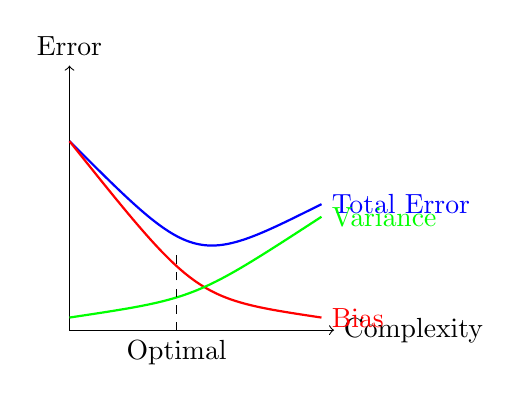
\begin{tikzpicture}[scale=0.8]
        \draw[->] (0,0) -- (4.2,0) node[right] {Complexity};
        \draw[->] (0,0) -- (0,4.2) node[above] {Error};
        \draw[thick, blue] (0,3) .. controls (2,1) .. (4,2) node[right] {Total Error};
        \draw[thick, red] (0,3) .. controls (2,0.5) .. (4,0.2) node[right] {Bias};
        \draw[thick, green] (0,0.2) .. controls (2,0.5) .. (4,1.8) node[right] {Variance};
        \draw[dashed] (1.7,0) -- (1.7,1.3);
        \node at (1.7,0) [below] {Optimal};
      \end{tikzpicture}
    \end{column}
  \end{columns}
\end{frame}

\begin{frame}{Estimating Parameters of a Gaussian Distribution}
  Given a sample $X_1, X_2, \ldots, X_n \sim \mathcal{N}(\mu, \sigma^2)$:
  
  \begin{block}{Maximum Likelihood Estimators}
    \begin{align*}
    \hat{\mu}_{\text{MLE}} &= \frac{1}{n} \sum_{i=1}^n X_i \\
    \hat{\sigma}^2_{\text{MLE}} &= \frac{1}{n} \sum_{i=1}^n (X_i - \hat{\mu}_{\text{MLE}})^2
    \end{align*}
  \end{block}
  
  \begin{block}{Properties}
    \begin{itemize}
      \item $\hat{\mu}_{\text{MLE}}$ is unbiased: $\mathbb{E}[\hat{\mu}_{\text{MLE}}] = \mu$
      \item $\hat{\sigma}^2_{\text{MLE}}$ is biased: $\mathbb{E}[\hat{\sigma}^2_{\text{MLE}}] = \frac{n-1}{n} \sigma^2$
      \item Unbiased variance estimator: $\hat{\sigma}^2_{\text{unbiased}} = \frac{1}{n-1} \sum_{i=1}^n (X_i - \hat{\mu})^2$
    \end{itemize}
  \end{block}
\end{frame}

\begin{frame}{Temperature Measurements: A Case Study}
  Suppose daily temperatures follow $\mathcal{N}(20^\circ\text{C}, 25\text{ }^\circ\text{C}^2)$:
  
  \begin{columns}
    \begin{column}{0.5\textwidth}
      \begin{block}{Small Sample ($n=10$)}
        \begin{align*}
        \hat{\mu} &= 18.5^\circ\text{C} \\
        \hat{\sigma}^2 &= 19.8\text{ }^\circ\text{C}^2
        \end{align*}
        \centerline{High bias, high variance}
      \end{block}
    \end{column}
    \begin{column}{0.5\textwidth}
      \begin{block}{Large Sample ($n=1000$)}
        \begin{align*}
        \hat{\mu} &= 20.1^\circ\text{C} \\
        \hat{\sigma}^2 &= 24.9\text{ }^\circ\text{C}^2
        \end{align*}
        \centerline{Low bias, low variance}
      \end{block}
    \end{column}
  \end{columns}
  
  \begin{block}{Sampling Distribution}
    $\hat{\mu} \sim \mathcal{N}\left(\mu, \frac{\sigma^2}{n}\right) = \mathcal{N}\left(20, \frac{25}{n}\right)$
  \end{block}
\end{frame}

\begin{frame}{Model Complexity: Underfitting vs. Overfitting}
  \begin{block}{Underfitting (High Bias)}
    \begin{itemize}
      \item Model is too simple to capture underlying structure
      \item Example: Linear model for seasonal temperature variation
      \item $f(x) = \beta_0 + \beta_1 x$
    \end{itemize}
  \end{block}
  
  \begin{block}{Good Fit (Balanced)}
    \begin{itemize}
      \item Model captures the main patterns without fitting noise
      \item Example: Cubic model for seasonal temperature
      \item $f(x) = \beta_0 + \beta_1 x + \beta_2 x^2 + \beta_3 x^3$
    \end{itemize}
  \end{block}
  
  \begin{block}{Overfitting (High Variance)}
    \begin{itemize}
      \item Model captures noise, not just underlying structure
      \item Example: 30-degree polynomial for temperature data
      \item Performs well on training data, poorly on new data
    \end{itemize}
  \end{block}
\end{frame}

\begin{frame}{Practical Techniques for Bias-Variance Management}
  \begin{block}{Regularization}
    \begin{itemize}
      \item \textbf{Ridge Regression}: L2 penalty, shrinks coefficients toward zero
      \item \textbf{Lasso Regression}: L1 penalty, performs feature selection
      \item \textbf{Elastic Net}: Combines L1 and L2 penalties
    \end{itemize}
  \end{block}
  
  \begin{block}{Cross-Validation}
    \begin{enumerate}
      \item Split data into $k$ folds
      \item For each model complexity:
      \begin{itemize}
        \item Train on $k-1$ folds, test on remaining fold
        \item Repeat for all folds and average results
      \end{itemize}
      \item Choose complexity with best validation performance
    \end{enumerate}
  \end{block}
\end{frame}

\begin{frame}{Practical Guidelines for Machine Learning}
  \begin{itemize}
    \item \textbf{Small datasets}: Use simpler models (prioritize variance reduction)
    \item \textbf{Large datasets}: Can use more complex models (focus on bias reduction)
    \item \textbf{Start simple}: Begin with simpler models and gradually increase complexity
    \item \textbf{Ensemble methods}:
    \begin{itemize}
      \item \textbf{Bagging} (Random Forests): Reduces variance
      \item \textbf{Boosting}: Reduces bias
      \item \textbf{Stacking}: Combines multiple models
    \end{itemize}
    \item \textbf{Feature selection}: Remove irrelevant features to reduce variance
    \item \textbf{Regularization}: Add constraints to control overfitting
  \end{itemize}
\end{frame}

\section{Conclusion}

\begin{frame}{Key Takeaways}
  \begin{itemize}
    \item The Gaussian distribution is mathematically elegant and computationally tractable
    \item The Central Limit Theorem explains its pervasiveness in natural phenomena
    \item Maximum Entropy Principle establishes its information-theoretic optimality
    \item Multivariate Gaussians have remarkable properties for marginal and conditional distributions
    \item The bias-variance decomposition helps understand prediction error
    \item The tradeoff between model complexity and performance is fundamental
    \item Regularization and cross-validation help manage the bias-variance tradeoff
  \end{itemize}
\end{frame}

\begin{frame}{Further Reading}
  \begin{itemize}
    \item Bishop, C. M. (2006). \textit{Pattern Recognition and Machine Learning}. Springer.
    \item Rasmussen, C. E., \& Williams, C. K. I. (2006). \textit{Gaussian Processes for Machine Learning}. MIT Press.
    \item Cover, T. M., \& Thomas, J. A. (2006). \textit{Elements of Information Theory}. Wiley-Interscience.
    \item Murphy, K. P. (2012). \textit{Machine Learning: A Probabilistic Perspective}. MIT Press.
    \item Hastie, T., Tibshirani, R., \& Friedman, J. (2009). \textit{The Elements of Statistical Learning}. Springer.
  \end{itemize}
\end{frame}

\end{document}